\documentclass[11pt,a4paper]{article}
\usepackage{latexsym}
\usepackage{graphicx}
\usepackage{amssymb,amsmath,url}
\usepackage{mathtools,braket}
\usepackage[english]{babel}
\usepackage{caption}
\usepackage{subcaption}
\usepackage{graphicx}

% Parametri di stampa
\setlength{\topmargin}{-2.5cm} \setlength{\oddsidemargin}{0.3cm}
\setlength{\evensidemargin}{0.3cm}
%
\textheight=23.0truecm \textwidth=16.0truecm
%
\headheight=1.0cm \headsep=1.0cm
%
\renewcommand{\baselinestretch}{1.1}
\setlength{\unitlength}{1mm}

\parindent=6pt

%%%%%%%%%%%%%%%%%%%%%%%%%%%%%%%%%%%%%%%%%%%%%%%%%%%%%%%%%%%%%%%%%%%%%%%%%%%%

\newcommand{\be}{\begin{equation}}
\newcommand{\ee}{\end{equation}}
\newcommand{\bea}{\begin{eqnarray}}
\newcommand{\eea}{\end{eqnarray}}

\newcommand{\op}[1]{\hat {#1}}

%%%%%%%%%%%%%%%%%%%%%%%%%%%%%%%%%%%%%%%%%%%%%%%%%%%%%%%%%%%%%%%%%%%%%%%%%%%%

\begin{document}

%%%%%%%%%%%%%%%%%%%%%%%%%%%%%%%%%%%%%%%%%%%%%%%%%%%%%%%%%%%%%%%%%%%%%%%%%%%%


\section*{Supplementary material}

We have investigated how the multi-threshold structure of the localized excitations might be put in relation with respect to
the number of atoms and/or the symmetry of the molecule. To this end, we have considered two case-studies, the carbon Fullerene, a highly symmetric structure made of 60 atoms, and the B1 Aflatoxin, depicted in Fig.~\ref{aflab1}, which has 35 atoms in a low-symmetric configuration.

The plots of Fig. \ref{exc-land} evidence that, in both cases, the sector of localized excitations is very rich and extends well above the first ionization potential of the molecule. These results provide a further confirmation of the behavior already observed in Table I.
\begin{figure}[h]
  \centering
  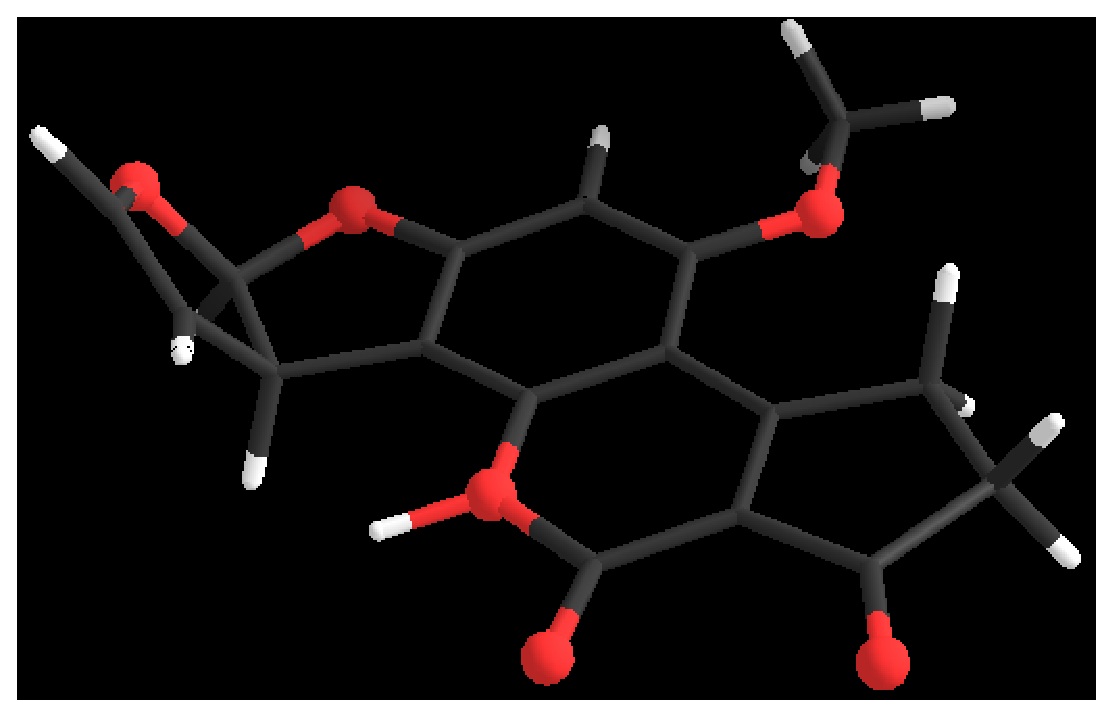
\includegraphics[width=0.4\textwidth]{AflaB1.eps}
    \caption{Equilibrium position of the Aflatoxin B1}
\label{aflab1}
\end{figure}

It may be noticed that the number of localized excitations, either below or above the first ionization potentials is much higher than
the one of Fig.~5 of the paper, in the case of the Benzene molecule. This holds also for the low-symmetry aflatoxin molecule.

The growth of the localized sector with the number of atoms of the molecule seems thus to be a general feature.
A simple interpretation of this fact may be provided by considering perturbatively the coupling term $\op V'=0$ in Eq.~19 of the paper.
Indeed, larger molecules possess a high number of localized Kohn-Sham (KS) orbitals that span a wide energy range.
A numerical evidence in support of this argument is presented in Fig. \ref{dos}, where the DOS of the KS (bound) orbitals of the Aflatoxin and $CO$ molecules are directly compared.

In a simplified two-orbitals picture, in which $\op V'=0$, the KS empty orbitals $\psi_a$ coincide with the excitation modes defined in eq. (17) and the associated energy is given by $\Omega_a=\epsilon_a-\epsilon_p$.
The increase of the KS DOS below the continuum threshold is therefore directly responsible of the increase of the number of localized excitations above IP.

 Such a two-orbital picture is of course not valid anymore when the coupling $\op V'$ is switched on. Yet, by interpreting perturbatively the action of the coupling term the same arguments hold true; larger molecule seem to have higher rate of  localized excitations as their DOS of KS bound states is higher.

 All the details of the calculations, the \textsl{Jupyter} notebooks of the data analysis of all the molecules considered in this study may be found at the URL~\url{https://github.com/luigigenovese/LR-nb/blob/master/POLARIZABILITY/nb_paper/LR_Analysis.ipynb}.

\begin{figure}[h]
    \centering
    \begin{subfigure}[t]{0.48\textwidth}
        \centering
        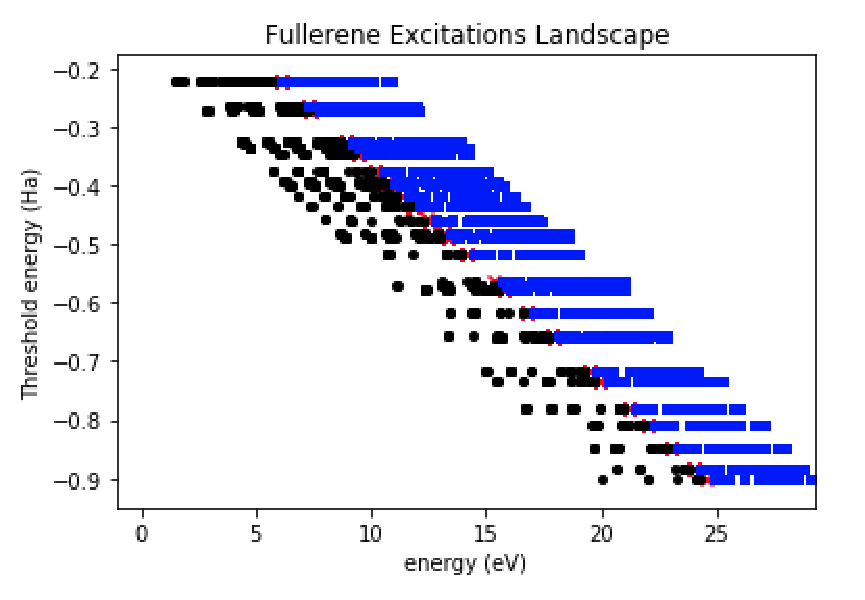
\includegraphics[width=\linewidth]{C60_ExcitationLandscape.eps}
        \caption{$C_{60}$} \label{fig:b}
    \end{subfigure}
    \hfill
    \begin{subfigure}[t]{0.48\textwidth}
        \centering
        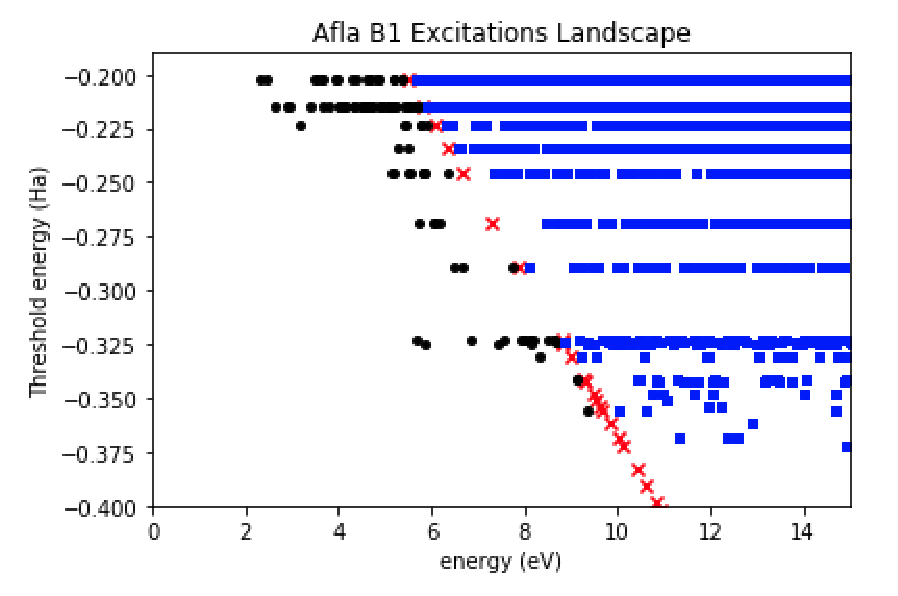
\includegraphics[width=\linewidth]{Aflatoxin_ExcitationLandscape.eps}
        \caption{Aflatoxin} \label{fig:a}
    \end{subfigure}
    \caption{Excitation landscape for the $C_{60}$ (panel a) and the Aflatoxin (panel b) molecules computed accordingly to the procedure described  in the appendix C. Black circles represent the localized sector and blue squares describe the pseudo-continuum one.}
\label{exc-land}
\end{figure}

\begin{figure}[h]
    \centering
    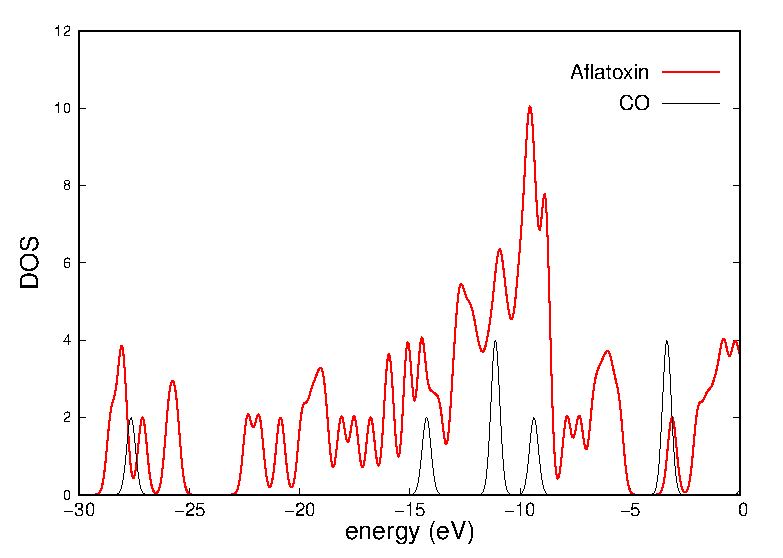
\includegraphics[width=9cm]{DOS_Afla&CO.eps}
    \caption{DOS of the (bound) KS states for the Aflatoxin and the $CO$ molecules. }
\label{dos}
\end{figure}



%%%%%%%%%%%%%%%%%%%%%%%%%%%%%%%%%%%%%%%%%%%%%%%%%%%%%%%%%%%%%%%%%%%%%%%%%%%%

\end{document}

%%%%%%%%%%%%%%%%%%%%%%%%%%%%%%%%%%%%%%%%%%%%%%%%%%%%%%%%%%%%%%%%%%%%%%%%%%%%
